\documentclass[1p]{elsarticle_modified}
%\bibliographystyle{elsarticle-num}

%\usepackage[colorlinks]{hyperref}
%\usepackage{abbrmath_seonhwa} %\Abb, \Ascr, \Acal ,\Abf, \Afrak
\usepackage{amsfonts}
\usepackage{amssymb}
\usepackage{amsmath}
\usepackage{amsthm}
\usepackage{scalefnt}
\usepackage{amsbsy}
\usepackage{kotex}
\usepackage{caption}
\usepackage{subfig}
\usepackage{color}
\usepackage{graphicx}
\usepackage{xcolor} %% white, black, red, green, blue, cyan, magenta, yellow
\usepackage{float}
\usepackage{setspace}
\usepackage{hyperref}

\usepackage{tikz}
\usetikzlibrary{arrows}

\usepackage{multirow}
\usepackage{array} % fixed length table
\usepackage{hhline}

%%%%%%%%%%%%%%%%%%%%%
\makeatletter
\renewcommand*\env@matrix[1][\arraystretch]{%
	\edef\arraystretch{#1}%
	\hskip -\arraycolsep
	\let\@ifnextchar\new@ifnextchar
	\array{*\c@MaxMatrixCols c}}
\makeatother %https://tex.stackexchange.com/questions/14071/how-can-i-increase-the-line-spacing-in-a-matrix
%%%%%%%%%%%%%%%

\usepackage[normalem]{ulem}

\newcommand{\msout}[1]{\ifmmode\text{\sout{\ensuremath{#1}}}\else\sout{#1}\fi}
%SOURCE: \msout is \stkout macro in https://tex.stackexchange.com/questions/20609/strikeout-in-math-mode

\newcommand{\cancel}[1]{
	\ifmmode
	{\color{red}\msout{#1}}
	\else
	{\color{red}\sout{#1}}
	\fi
}

\newcommand{\add}[1]{
	{\color{blue}\uwave{#1}}
}

\newcommand{\replace}[2]{
	\ifmmode
	{\color{red}\msout{#1}}{\color{blue}\uwave{#2}}
	\else
	{\color{red}\sout{#1}}{\color{blue}\uwave{#2}}
	\fi
}

\newcommand{\Sol}{\mathcal{S}} %segment
\newcommand{\D}{D} %diagram
\newcommand{\A}{\mathcal{A}} %arc


%%%%%%%%%%%%%%%%%%%%%%%%%%%%%5 test

\def\sl{\operatorname{\textup{SL}}(2,\Cbb)}
\def\psl{\operatorname{\textup{PSL}}(2,\Cbb)}
\def\quan{\mkern 1mu \triangleright \mkern 1mu}

\theoremstyle{definition}
\newtheorem{thm}{Theorem}[section]
\newtheorem{prop}[thm]{Proposition}
\newtheorem{lem}[thm]{Lemma}
\newtheorem{ques}[thm]{Question}
\newtheorem{cor}[thm]{Corollary}
\newtheorem{defn}[thm]{Definition}
\newtheorem{exam}[thm]{Example}
\newtheorem{rmk}[thm]{Remark}
\newtheorem{alg}[thm]{Algorithm}

\newcommand{\I}{\sqrt{-1}}
\begin{document}

%\begin{frontmatter}
%
%\title{Boundary parabolic representations of knots up to 8 crossings}
%
%%% Group authors per affiliation:
%\author{Yunhi Cho} 
%\address{Department of Mathematics, University of Seoul, Seoul, Korea}
%\ead{yhcho@uos.ac.kr}
%
%
%\author{Seonhwa Kim} %\fnref{s_kim}}
%\address{Center for Geometry and Physics, Institute for Basic Science, Pohang, 37673, Korea}
%\ead{ryeona17@ibs.re.kr}
%
%\author{Hyuk Kim}
%\address{Department of Mathematical Sciences, Seoul National University, Seoul 08826, Korea}
%\ead{hyukkim@snu.ac.kr}
%
%\author{Seokbeom Yoon}
%\address{Department of Mathematical Sciences, Seoul National University, Seoul, 08826,  Korea}
%\ead{sbyoon15@snu.ac.kr}
%
%\begin{abstract}
%We find all boundary parabolic representation of knots up to 8 crossings.
%
%\end{abstract}
%\begin{keyword}
%    \MSC[2010] 57M25 
%\end{keyword}
%
%\end{frontmatter}

%\linenumbers
%\tableofcontents
%
\newcommand\colored[1]{\textcolor{white}{\rule[-0.35ex]{0.8em}{1.4ex}}\kern-0.8em\color{red} #1}%
%\newcommand\colored[1]{\textcolor{white}{ #1}\kern-2.17ex	\textcolor{white}{ #1}\kern-1.81ex	\textcolor{white}{ #1}\kern-2.15ex\color{red}#1	}

{\Large $\underline{11n_{81}~(K11n_{81})}$}

\setlength{\tabcolsep}{10pt}
\renewcommand{\arraystretch}{1.6}
\vspace{1cm}\begin{tabular}{m{100pt}>{\centering\arraybackslash}m{274pt}}
\multirow{5}{120pt}{
	\centering
	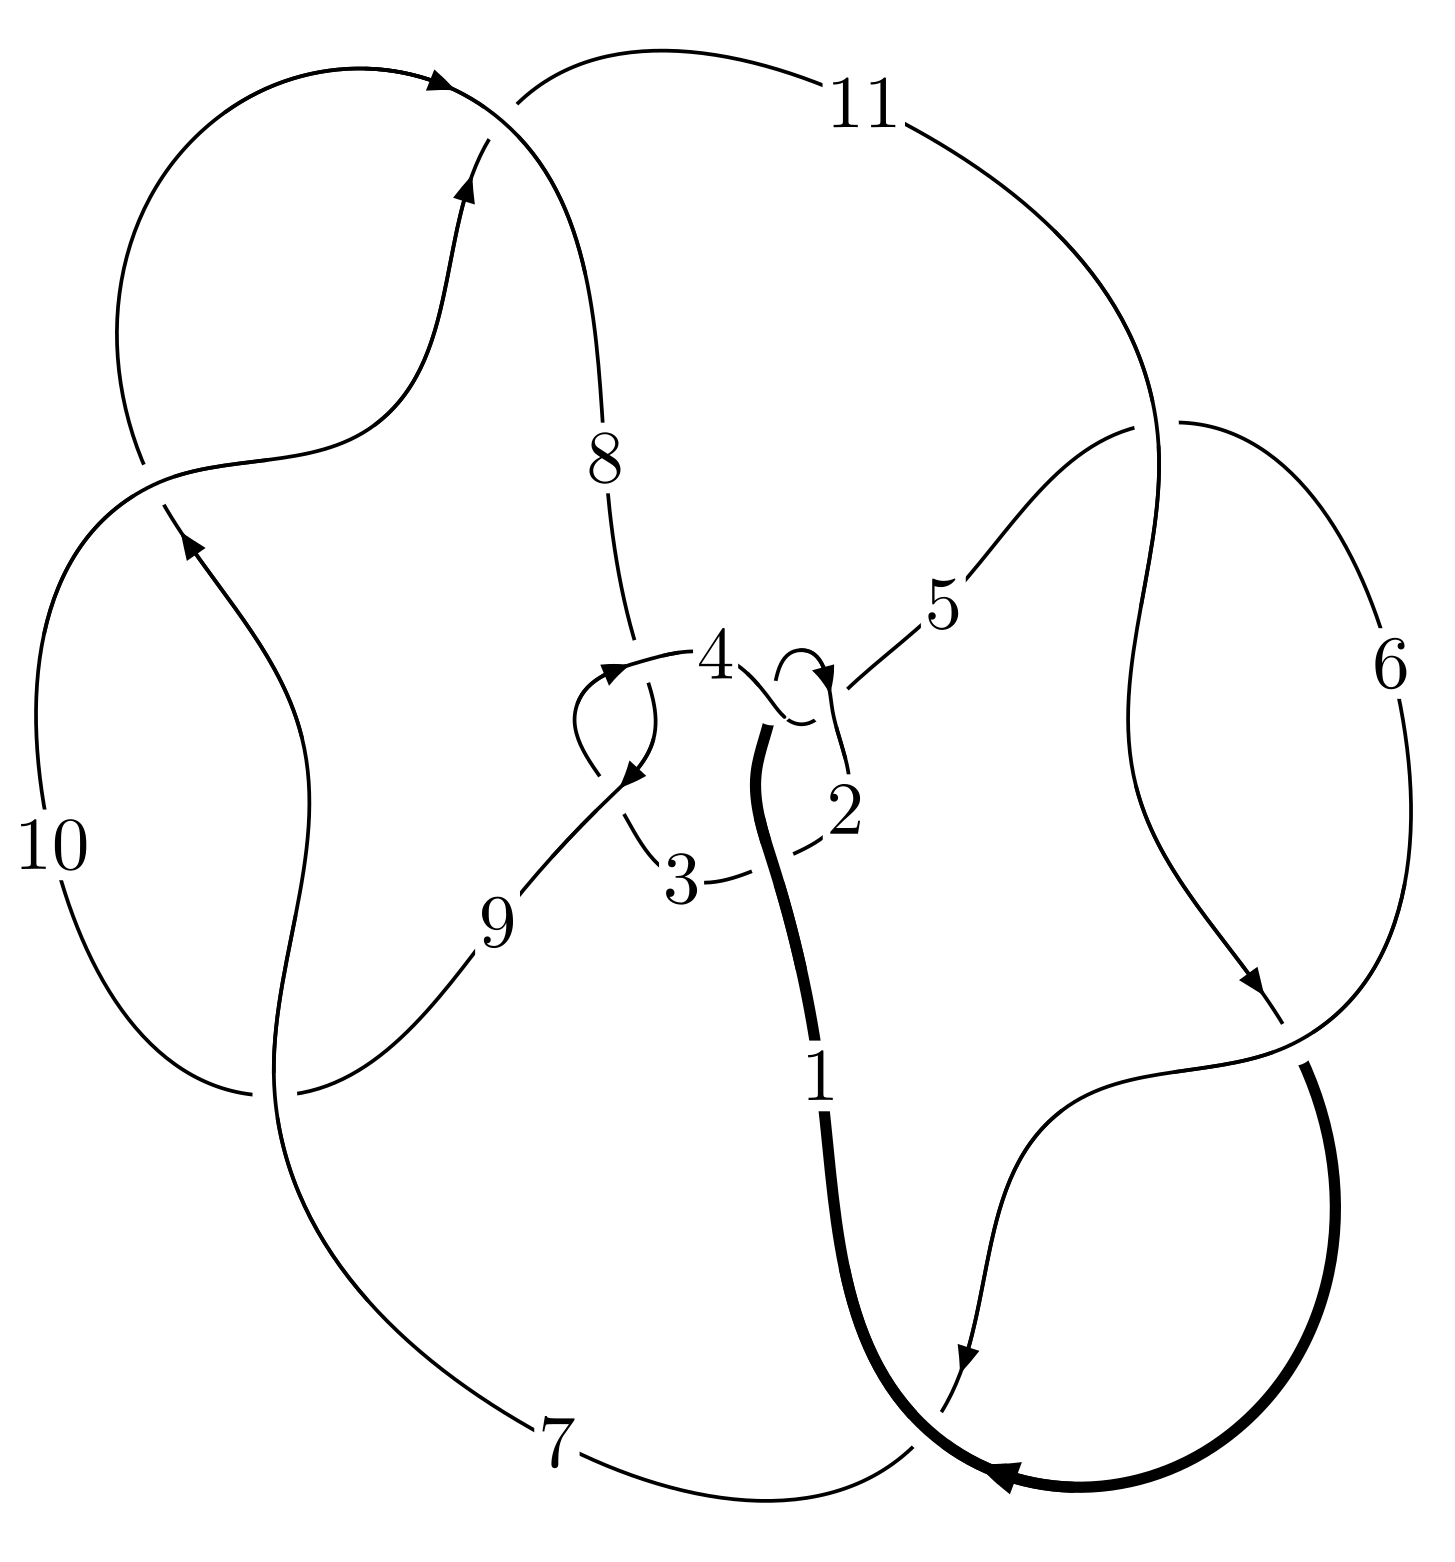
\includegraphics[width=112pt]{../../../GIT/diagram.site/Diagrams/png/697_11n_81.png}\\
\ \ \ A knot diagram\footnotemark}&
\allowdisplaybreaks
\textbf{Linearized knot diagam} \\
\cline{2-2}
 &
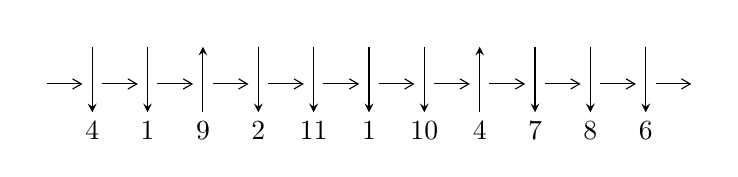
\begin{tikzpicture}[x=20pt, y=17pt]
	% nodes
	\node (C0) at (0, 0) {};
	\node (C1) at (1, 0) {};
	\node (C1U) at (1, +1) {};
	\node (C1D) at (1, -1) {4};

	\node (C2) at (2, 0) {};
	\node (C2U) at (2, +1) {};
	\node (C2D) at (2, -1) {1};

	\node (C3) at (3, 0) {};
	\node (C3U) at (3, +1) {};
	\node (C3D) at (3, -1) {9};

	\node (C4) at (4, 0) {};
	\node (C4U) at (4, +1) {};
	\node (C4D) at (4, -1) {2};

	\node (C5) at (5, 0) {};
	\node (C5U) at (5, +1) {};
	\node (C5D) at (5, -1) {11};

	\node (C6) at (6, 0) {};
	\node (C6U) at (6, +1) {};
	\node (C6D) at (6, -1) {1};

	\node (C7) at (7, 0) {};
	\node (C7U) at (7, +1) {};
	\node (C7D) at (7, -1) {10};

	\node (C8) at (8, 0) {};
	\node (C8U) at (8, +1) {};
	\node (C8D) at (8, -1) {4};

	\node (C9) at (9, 0) {};
	\node (C9U) at (9, +1) {};
	\node (C9D) at (9, -1) {7};

	\node (C10) at (10, 0) {};
	\node (C10U) at (10, +1) {};
	\node (C10D) at (10, -1) {8};

	\node (C11) at (11, 0) {};
	\node (C11U) at (11, +1) {};
	\node (C11D) at (11, -1) {6};
	\node (C12) at (12, 0) {};

	% arrows
	\draw[->,>={angle 60}]
	(C0) edge (C1) (C1) edge (C2) (C2) edge (C3) (C3) edge (C4) (C4) edge (C5) (C5) edge (C6) (C6) edge (C7) (C7) edge (C8) (C8) edge (C9) (C9) edge (C10) (C10) edge (C11) (C11) edge (C12) ;	\draw[->,>=stealth]
	(C1U) edge (C1D) (C2U) edge (C2D) (C3D) edge (C3U) (C4U) edge (C4D) (C5U) edge (C5D) (C6U) edge (C6D) (C7U) edge (C7D) (C8D) edge (C8U) (C9U) edge (C9D) (C10U) edge (C10D) (C11U) edge (C11D) ;
	\end{tikzpicture} \\
\hhline{~~} \\& 
\textbf{Solving Sequence} \\ \cline{2-2} 
 &
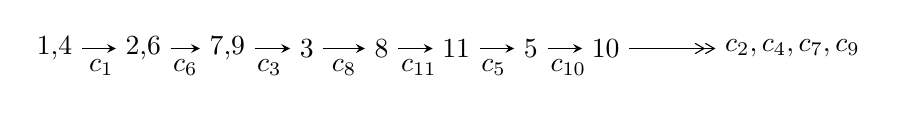
\begin{tikzpicture}[x=27pt, y=7pt]
	% node
	\node (A0) at (-1/8, 0) {1,4};
	\node (A1) at (17/16, 0) {2,6};
	\node (A2) at (35/16, 0) {7,9};
	\node (A3) at (13/4, 0) {3};
	\node (A4) at (17/4, 0) {8};
	\node (A5) at (21/4, 0) {11};
	\node (A6) at (25/4, 0) {5};
	\node (A7) at (29/4, 0) {10};
	\node (C1) at (1/2, -1) {$c_{1}$};
	\node (C2) at (13/8, -1) {$c_{6}$};
	\node (C3) at (11/4, -1) {$c_{3}$};
	\node (C4) at (15/4, -1) {$c_{8}$};
	\node (C5) at (19/4, -1) {$c_{11}$};
	\node (C6) at (23/4, -1) {$c_{5}$};
	\node (C7) at (27/4, -1) {$c_{10}$};
	\node (A8) at (39/4, 0) {$c_{2},c_{4},c_{7},c_{9}$};

	% edge
	\draw[->,>=stealth]	
	(A0) edge (A1) (A1) edge (A2) (A2) edge (A3) (A3) edge (A4) (A4) edge (A5) (A5) edge (A6) (A6) edge (A7) ;
	\draw[->>,>={angle 60}]	
	(A7) edge (A8);
\end{tikzpicture} \\ 

\end{tabular} \\

\footnotetext{
The image of knot diagram is generated by the software ``\textbf{Draw programme}" developed by Andrew Bartholomew(\url{http://www.layer8.co.uk/maths/draw/index.htm\#Running-draw}), where we modified some parts for our purpose(\url{https://github.com/CATsTAILs/LinksPainter}).
}\phantom \\ \newline 
\centering \textbf{Ideals for irreducible components\footnotemark of $X_{\text{par}}$} 
 
\begin{align*}
I^u_{1}&=\langle 
- u^3+u^2+2 d+3 u-1,\;u^4+2 u^3-4 u^2+2 c-8 u+1,\;b- u,\;- u^4- u^3+3 u^2+2 a+3 u,\\
\phantom{I^u_{1}}&\phantom{= \langle  }u^5+u^4-4 u^3-4 u^2+3 u-1\rangle \\
I^u_{2}&=\langle 
- u^4+2 u^2+d-2 u,\;u^4+u^3-2 u^2+c+2,\;b- u,\;u^3+2 u^2+a- u-1,\;u^5+2 u^4-2 u^3-3 u^2+3 u+1\rangle \\
I^u_{3}&=\langle 
- u^4+2 u^2+d-2 u,\;u^4+u^3-2 u^2+c+2,\;- u^4- u^3+2 u^2+b+u-1,\;- u^4-2 u^3+2 u^2+a+3 u-3,\\
\phantom{I^u_{3}}&\phantom{= \langle  }u^5+2 u^4-2 u^3-3 u^2+3 u+1\rangle \\
I^u_{4}&=\langle 
-5 u^4+6 u^3-3 u^2+4 d-9 u+14,\;3 u^4-2 u^3+u^2+8 c+3 u-10,\;u^4-2 u^3- u^2+4 b+5 u-2,\\
\phantom{I^u_{4}}&\phantom{= \langle  }u^4- u^2+4 a+3 u,\;u^5- u^3+3 u^2-4\rangle \\
I^u_{5}&=\langle 
d+1,\;c,\;b,\;a+1,\;u-1\rangle \\
I^u_{6}&=\langle 
d+1,\;c,\;b+1,\;a+1,\;u-1\rangle \\
I^u_{7}&=\langle 
d a+d+1,\;c,\;b+1,\;u-1\rangle \\
\\
I^v_{1}&=\langle 
a,\;d,\;c+1,\;b-1,\;v-1\rangle \\
\end{align*}
\raggedright * 7 irreducible components of $\dim_{\mathbb{C}}=0$, with total 23 representations.\\
\raggedright * 1 irreducible components of $\dim_{\mathbb{C}}=1$ \\
\footnotetext{All coefficients of polynomials are rational numbers. But the coefficients are sometimes approximated in decimal forms when there is not enough margin.}
\newpage
\renewcommand{\arraystretch}{1}
\centering \section*{I. $I^u_{1}= \langle - u^3+u^2+2 d+3 u-1,\;u^4+2 u^3+\cdots+2 c+1,\;b- u,\;- u^4- u^3+3 u^2+2 a+3 u,\;u^5+u^4+\cdots+3 u-1 \rangle$}
\flushleft \textbf{(i) Arc colorings}\\
\begin{tabular}{m{7pt} m{180pt} m{7pt} m{180pt} }
\flushright $a_{1}=$&$\begin{pmatrix}1\\0\end{pmatrix}$ \\
\flushright $a_{4}=$&$\begin{pmatrix}0\\u\end{pmatrix}$ \\
\flushright $a_{2}=$&$\begin{pmatrix}1\\u^2\end{pmatrix}$ \\
\flushright $a_{6}=$&$\begin{pmatrix}\frac{1}{2} u^4+\frac{1}{2} u^3-\frac{3}{2} u^2-\frac{3}{2} u\\u\end{pmatrix}$ \\
\flushright $a_{7}=$&$\begin{pmatrix}\frac{1}{2} u^4+\frac{1}{2} u^3-\frac{3}{2} u^2-\frac{5}{2} u\\u\end{pmatrix}$ \\
\flushright $a_{9}=$&$\begin{pmatrix}-\frac{1}{2} u^4- u^3+2 u^2+4 u-\frac{1}{2}\\\frac{1}{2} u^3-\frac{1}{2} u^2-\frac{3}{2} u+\frac{1}{2}\end{pmatrix}$ \\
\flushright $a_{3}=$&$\begin{pmatrix}- u^2+1\\u^2\end{pmatrix}$ \\
\flushright $a_{8}=$&$\begin{pmatrix}-\frac{1}{2} u^4- u^3+2 u^2+4 u-\frac{1}{2}\\\frac{1}{2} u^4+\frac{1}{2} u^3-\frac{3}{2} u^2-\frac{1}{2} u\end{pmatrix}$ \\
\flushright $a_{11}=$&$\begin{pmatrix}-\frac{1}{2} u^3-\frac{1}{2} u^2+\frac{3}{2} u+\frac{1}{2}\\- u^2\end{pmatrix}$ \\
\flushright $a_{5}=$&$\begin{pmatrix}- u\\- u^3+u\end{pmatrix}$ \\
\flushright $a_{10}=$&$\begin{pmatrix}-\frac{1}{2} u^4-\frac{1}{2} u^3+\frac{3}{2} u^2+\frac{5}{2} u\\\frac{1}{2} u^3+\frac{1}{2} u^2-\frac{3}{2} u+\frac{1}{2}\end{pmatrix}$\\ \flushright $a_{10}=$&$\begin{pmatrix}-\frac{1}{2} u^4-\frac{1}{2} u^3+\frac{3}{2} u^2+\frac{5}{2} u\\\frac{1}{2} u^3+\frac{1}{2} u^2-\frac{3}{2} u+\frac{1}{2}\end{pmatrix}$\\&\end{tabular}
\flushleft \textbf{(ii) Obstruction class $= -1$}\\~\\
\flushleft \textbf{(iii) Cusp Shapes $= -3 u^4-6 u^3+10 u^2+22 u-13$}\\~\\
\newpage\renewcommand{\arraystretch}{1}
\flushleft \textbf{(iv) u-Polynomials at the component}\newline \\
\begin{tabular}{m{50pt}|m{274pt}}
Crossings & \hspace{64pt}u-Polynomials at each crossing \\
\hline $$\begin{aligned}c_{1},c_{4},c_{5}\\c_{6},c_{7},c_{9}\\c_{10},c_{11}\end{aligned}$$&$\begin{aligned}
&u^5- u^4-4 u^3+4 u^2+3 u+1
\end{aligned}$\\
\hline $$\begin{aligned}c_{2}\end{aligned}$$&$\begin{aligned}
&u^5+9 u^4+30 u^3+38 u^2+u+1
\end{aligned}$\\
\hline $$\begin{aligned}c_{3},c_{8}\end{aligned}$$&$\begin{aligned}
&u^5+4 u^4+8 u^3+8 u^2+4
\end{aligned}$\\
\hline
\end{tabular}\\~\\
\newpage\renewcommand{\arraystretch}{1}
\flushleft \textbf{(v) Riley Polynomials at the component}\newline \\
\begin{tabular}{m{50pt}|m{274pt}}
Crossings & \hspace{64pt}Riley Polynomials at each crossing \\
\hline $$\begin{aligned}c_{1},c_{4},c_{5}\\c_{6},c_{7},c_{9}\\c_{10},c_{11}\end{aligned}$$&$\begin{aligned}
&y^5-9 y^4+30 y^3-38 y^2+y-1
\end{aligned}$\\
\hline $$\begin{aligned}c_{2}\end{aligned}$$&$\begin{aligned}
&y^5-21 y^4+218 y^3-1402 y^2-75 y-1
\end{aligned}$\\
\hline $$\begin{aligned}c_{3},c_{8}\end{aligned}$$&$\begin{aligned}
&y^5-96 y^2-64 y-16
\end{aligned}$\\
\hline
\end{tabular}\\~\\
\newpage\flushleft \textbf{(vi) Complex Volumes and Cusp Shapes}
$$\begin{array}{c|c|c}  
\text{Solutions to }I^u_{1}& \I (\text{vol} + \sqrt{-1}CS) & \text{Cusp shape}\\
 \hline 
\begin{aligned}
u &= \phantom{-}0.287923 + 0.283171 I \\
a &= -0.471944 - 0.645049 I \\
b &= \phantom{-}0.287923 + 0.283171 I \\
c &= \phantom{-}0.71581 + 1.41065 I \\
d &= \phantom{-}0.044061 - 0.482429 I\end{aligned}
 & -0.341586 - 0.921914 I & -6.28644 + 7.57142 I \\ \hline\begin{aligned}
u &= \phantom{-}0.287923 - 0.283171 I \\
a &= -0.471944 + 0.645049 I \\
b &= \phantom{-}0.287923 - 0.283171 I \\
c &= \phantom{-}0.71581 - 1.41065 I \\
d &= \phantom{-}0.044061 + 0.482429 I\end{aligned}
 & -0.341586 + 0.921914 I & -6.28644 - 7.57142 I \\ \hline\begin{aligned}
u &= -1.72935 + 0.51571 I \\
a &= -1.26784 - 0.71317 I \\
b &= -1.72935 + 0.51571 I \\
c &= -0.297131 - 1.134290 I \\
d &= -0.16439 + 2.36316 I\end{aligned}
 & \phantom{-}16.6614 + 10.9560 I & -13.7735 - 4.2698 I \\ \hline\begin{aligned}
u &= -1.72935 - 0.51571 I \\
a &= -1.26784 + 0.71317 I \\
b &= -1.72935 - 0.51571 I \\
c &= -0.297131 + 1.134290 I \\
d &= -0.16439 - 2.36316 I\end{aligned}
 & \phantom{-}16.6614 - 10.9560 I & -13.7735 + 4.2698 I \\ \hline\begin{aligned}
u &= \phantom{-}1.88286\phantom{ +0.000000I} \\
a &= \phantom{-}1.47956\phantom{ +0.000000I} \\
b &= \phantom{-}1.88286\phantom{ +0.000000I} \\
c &= \phantom{-}1.16265\phantom{ +0.000000I} \\
d &= -0.759351\phantom{ +0.000000I}\end{aligned}
 & -17.8353\phantom{ +0.000000I} & -13.8800\phantom{ +0.000000I}\\
 \hline 
 \end{array}$$\newpage\newpage\renewcommand{\arraystretch}{1}
\centering \section*{II. $I^u_{2}= \langle - u^4+2 u^2+d-2 u,\;u^4+u^3-2 u^2+c+2,\;b- u,\;u^3+2 u^2+a- u-1,\;u^5+2 u^4+\cdots+3 u+1 \rangle$}
\flushleft \textbf{(i) Arc colorings}\\
\begin{tabular}{m{7pt} m{180pt} m{7pt} m{180pt} }
\flushright $a_{1}=$&$\begin{pmatrix}1\\0\end{pmatrix}$ \\
\flushright $a_{4}=$&$\begin{pmatrix}0\\u\end{pmatrix}$ \\
\flushright $a_{2}=$&$\begin{pmatrix}1\\u^2\end{pmatrix}$ \\
\flushright $a_{6}=$&$\begin{pmatrix}- u^3-2 u^2+u+1\\u\end{pmatrix}$ \\
\flushright $a_{7}=$&$\begin{pmatrix}- u^3-2 u^2+1\\u\end{pmatrix}$ \\
\flushright $a_{9}=$&$\begin{pmatrix}- u^4- u^3+2 u^2-2\\u^4-2 u^2+2 u\end{pmatrix}$ \\
\flushright $a_{3}=$&$\begin{pmatrix}- u^2+1\\u^2\end{pmatrix}$ \\
\flushright $a_{8}=$&$\begin{pmatrix}- u^4- u^3+2 u^2-2\\- u^4- u^3+2 u^2-1\end{pmatrix}$ \\
\flushright $a_{11}=$&$\begin{pmatrix}u^4+2 u^3- u^2- u+1\\- u^2\end{pmatrix}$ \\
\flushright $a_{5}=$&$\begin{pmatrix}- u\\- u^3+u\end{pmatrix}$ \\
\flushright $a_{10}=$&$\begin{pmatrix}u^3+2 u^2-1\\-1\end{pmatrix}$\\ \flushright $a_{10}=$&$\begin{pmatrix}u^3+2 u^2-1\\-1\end{pmatrix}$\\&\end{tabular}
\flushleft \textbf{(ii) Obstruction class $= -1$}\\~\\
\flushleft \textbf{(iii) Cusp Shapes $= 4 u^4+6 u^3-8 u^2-6 u-4$}\\~\\
\newpage\renewcommand{\arraystretch}{1}
\flushleft \textbf{(iv) u-Polynomials at the component}\newline \\
\begin{tabular}{m{50pt}|m{274pt}}
Crossings & \hspace{64pt}u-Polynomials at each crossing \\
\hline $$\begin{aligned}c_{1},c_{4},c_{5}\\c_{6},c_{11}\end{aligned}$$&$\begin{aligned}
&u^5-2 u^4-2 u^3+3 u^2+3 u-1
\end{aligned}$\\
\hline $$\begin{aligned}c_{2}\end{aligned}$$&$\begin{aligned}
&u^5+8 u^4+22 u^3+25 u^2+15 u+1
\end{aligned}$\\
\hline $$\begin{aligned}c_{3},c_{8}\end{aligned}$$&$\begin{aligned}
&u^5- u^4+5 u^3- u^2+2 u+2
\end{aligned}$\\
\hline $$\begin{aligned}c_{7},c_{9},c_{10}\end{aligned}$$&$\begin{aligned}
&u^5- u^3-3 u^2+4
\end{aligned}$\\
\hline
\end{tabular}\\~\\
\newpage\renewcommand{\arraystretch}{1}
\flushleft \textbf{(v) Riley Polynomials at the component}\newline \\
\begin{tabular}{m{50pt}|m{274pt}}
Crossings & \hspace{64pt}Riley Polynomials at each crossing \\
\hline $$\begin{aligned}c_{1},c_{4},c_{5}\\c_{6},c_{11}\end{aligned}$$&$\begin{aligned}
&y^5-8 y^4+22 y^3-25 y^2+15 y-1
\end{aligned}$\\
\hline $$\begin{aligned}c_{2}\end{aligned}$$&$\begin{aligned}
&y^5-20 y^4+114 y^3+19 y^2+175 y-1
\end{aligned}$\\
\hline $$\begin{aligned}c_{3},c_{8}\end{aligned}$$&$\begin{aligned}
&y^5+9 y^4+27 y^3+23 y^2+8 y-4
\end{aligned}$\\
\hline $$\begin{aligned}c_{7},c_{9},c_{10}\end{aligned}$$&$\begin{aligned}
&y^5-2 y^4+y^3-9 y^2+24 y-16
\end{aligned}$\\
\hline
\end{tabular}\\~\\
\newpage\flushleft \textbf{(vi) Complex Volumes and Cusp Shapes}
$$\begin{array}{c|c|c}  
\text{Solutions to }I^u_{2}& \I (\text{vol} + \sqrt{-1}CS) & \text{Cusp shape}\\
 \hline 
\begin{aligned}
u &= \phantom{-}0.949895 + 0.441667 I \\
a &= \phantom{-}0.23423 - 2.34588 I \\
b &= \phantom{-}0.949895 + 0.441667 I \\
c &= -0.682871 - 0.618084 I \\
d &= \phantom{-}0.281458 + 0.392024 I\end{aligned}
 & -5.14125 - 1.10891 I & -14.3655 + 2.0411 I \\ \hline\begin{aligned}
u &= \phantom{-}0.949895 - 0.441667 I \\
a &= \phantom{-}0.23423 + 2.34588 I \\
b &= \phantom{-}0.949895 - 0.441667 I \\
c &= -0.682871 + 0.618084 I \\
d &= \phantom{-}0.281458 - 0.392024 I\end{aligned}
 & -5.14125 + 1.10891 I & -14.3655 - 2.0411 I \\ \hline\begin{aligned}
u &= -0.274898\phantom{ +0.000000I} \\
a &= \phantom{-}0.594739\phantom{ +0.000000I} \\
b &= -0.274898\phantom{ +0.000000I} \\
c &= -1.83380\phantom{ +0.000000I} \\
d &= -0.695222\phantom{ +0.000000I}\end{aligned}
 & -2.08622\phantom{ +0.000000I} & -3.05700\phantom{ +0.000000I} \\ \hline\begin{aligned}
u &= -1.81245 + 0.17314 I \\
a &= -1.53160 - 0.27272 I \\
b &= -1.81245 + 0.17314 I \\
c &= \phantom{-}0.099771 + 1.129450 I \\
d &= \phantom{-}0.06615 - 2.48427 I\end{aligned}
 & -15.1998 + 4.1249 I & -13.10604 - 2.15443 I \\ \hline\begin{aligned}
u &= -1.81245 - 0.17314 I \\
a &= -1.53160 + 0.27272 I \\
b &= -1.81245 - 0.17314 I \\
c &= \phantom{-}0.099771 - 1.129450 I \\
d &= \phantom{-}0.06615 + 2.48427 I\end{aligned}
 & -15.1998 - 4.1249 I & -13.10604 + 2.15443 I\\
 \hline 
 \end{array}$$\newpage\newpage\renewcommand{\arraystretch}{1}
\centering \section*{III. $I^u_{3}= \langle - u^4+2 u^2+d-2 u,\;u^4+u^3-2 u^2+c+2,\;- u^4- u^3+\cdots+b-1,\;- u^4-2 u^3+\cdots+a-3,\;u^5+2 u^4+\cdots+3 u+1 \rangle$}
\flushleft \textbf{(i) Arc colorings}\\
\begin{tabular}{m{7pt} m{180pt} m{7pt} m{180pt} }
\flushright $a_{1}=$&$\begin{pmatrix}1\\0\end{pmatrix}$ \\
\flushright $a_{4}=$&$\begin{pmatrix}0\\u\end{pmatrix}$ \\
\flushright $a_{2}=$&$\begin{pmatrix}1\\u^2\end{pmatrix}$ \\
\flushright $a_{6}=$&$\begin{pmatrix}u^4+2 u^3-2 u^2-3 u+3\\u^4+u^3-2 u^2- u+1\end{pmatrix}$ \\
\flushright $a_{7}=$&$\begin{pmatrix}u^3-2 u+2\\u^4+u^3-2 u^2- u+1\end{pmatrix}$ \\
\flushright $a_{9}=$&$\begin{pmatrix}- u^4- u^3+2 u^2-2\\u^4-2 u^2+2 u\end{pmatrix}$ \\
\flushright $a_{3}=$&$\begin{pmatrix}- u^2+1\\u^2\end{pmatrix}$ \\
\flushright $a_{8}=$&$\begin{pmatrix}- u^4- u^3+2 u^2-2\\- u^4- u^3+2 u^2-1\end{pmatrix}$ \\
\flushright $a_{11}=$&$\begin{pmatrix}- u^4- u^3+3 u^2+u-3\\- u^4+3 u^2-2 u-2\end{pmatrix}$ \\
\flushright $a_{5}=$&$\begin{pmatrix}- u\\- u^3+u\end{pmatrix}$ \\
\flushright $a_{10}=$&$\begin{pmatrix}- u^3+2 u-2\\-1\end{pmatrix}$\\ \flushright $a_{10}=$&$\begin{pmatrix}- u^3+2 u-2\\-1\end{pmatrix}$\\&\end{tabular}
\flushleft \textbf{(ii) Obstruction class $= -1$}\\~\\
\flushleft \textbf{(iii) Cusp Shapes $= 4 u^4+6 u^3-8 u^2-6 u-4$}\\~\\
\newpage\renewcommand{\arraystretch}{1}
\flushleft \textbf{(iv) u-Polynomials at the component}\newline \\
\begin{tabular}{m{50pt}|m{274pt}}
Crossings & \hspace{64pt}u-Polynomials at each crossing \\
\hline $$\begin{aligned}c_{1},c_{4},c_{7}\\c_{9},c_{10}\end{aligned}$$&$\begin{aligned}
&u^5-2 u^4-2 u^3+3 u^2+3 u-1
\end{aligned}$\\
\hline $$\begin{aligned}c_{2}\end{aligned}$$&$\begin{aligned}
&u^5+8 u^4+22 u^3+25 u^2+15 u+1
\end{aligned}$\\
\hline $$\begin{aligned}c_{3},c_{8}\end{aligned}$$&$\begin{aligned}
&u^5- u^4+5 u^3- u^2+2 u+2
\end{aligned}$\\
\hline $$\begin{aligned}c_{5},c_{6},c_{11}\end{aligned}$$&$\begin{aligned}
&u^5- u^3-3 u^2+4
\end{aligned}$\\
\hline
\end{tabular}\\~\\
\newpage\renewcommand{\arraystretch}{1}
\flushleft \textbf{(v) Riley Polynomials at the component}\newline \\
\begin{tabular}{m{50pt}|m{274pt}}
Crossings & \hspace{64pt}Riley Polynomials at each crossing \\
\hline $$\begin{aligned}c_{1},c_{4},c_{7}\\c_{9},c_{10}\end{aligned}$$&$\begin{aligned}
&y^5-8 y^4+22 y^3-25 y^2+15 y-1
\end{aligned}$\\
\hline $$\begin{aligned}c_{2}\end{aligned}$$&$\begin{aligned}
&y^5-20 y^4+114 y^3+19 y^2+175 y-1
\end{aligned}$\\
\hline $$\begin{aligned}c_{3},c_{8}\end{aligned}$$&$\begin{aligned}
&y^5+9 y^4+27 y^3+23 y^2+8 y-4
\end{aligned}$\\
\hline $$\begin{aligned}c_{5},c_{6},c_{11}\end{aligned}$$&$\begin{aligned}
&y^5-2 y^4+y^3-9 y^2+24 y-16
\end{aligned}$\\
\hline
\end{tabular}\\~\\
\newpage\flushleft \textbf{(vi) Complex Volumes and Cusp Shapes}
$$\begin{array}{c|c|c}  
\text{Solutions to }I^u_{3}& \I (\text{vol} + \sqrt{-1}CS) & \text{Cusp shape}\\
 \hline 
\begin{aligned}
u &= \phantom{-}0.949895 + 0.441667 I \\
a &= -0.865610 + 0.402477 I \\
b &= -1.267020 + 0.176417 I \\
c &= -0.682871 - 0.618084 I \\
d &= \phantom{-}0.281458 + 0.392024 I\end{aligned}
 & -5.14125 - 1.10891 I & -14.3655 + 2.0411 I \\ \hline\begin{aligned}
u &= \phantom{-}0.949895 - 0.441667 I \\
a &= -0.865610 - 0.402477 I \\
b &= -1.267020 - 0.176417 I \\
c &= -0.682871 + 0.618084 I \\
d &= \phantom{-}0.281458 - 0.392024 I\end{aligned}
 & -5.14125 + 1.10891 I & -14.3655 - 2.0411 I \\ \hline\begin{aligned}
u &= -0.274898\phantom{ +0.000000I} \\
a &= \phantom{-}3.63772\phantom{ +0.000000I} \\
b &= \phantom{-}1.10870\phantom{ +0.000000I} \\
c &= -1.83380\phantom{ +0.000000I} \\
d &= -0.695222\phantom{ +0.000000I}\end{aligned}
 & -2.08622\phantom{ +0.000000I} & -3.05700\phantom{ +0.000000I} \\ \hline\begin{aligned}
u &= -1.81245 + 0.17314 I \\
a &= \phantom{-}0.546751 + 0.052231 I \\
b &= \phantom{-}0.71268 - 1.30259 I \\
c &= \phantom{-}0.099771 + 1.129450 I \\
d &= \phantom{-}0.06615 - 2.48427 I\end{aligned}
 & -15.1998 + 4.1249 I & -13.10604 - 2.15443 I \\ \hline\begin{aligned}
u &= -1.81245 - 0.17314 I \\
a &= \phantom{-}0.546751 - 0.052231 I \\
b &= \phantom{-}0.71268 + 1.30259 I \\
c &= \phantom{-}0.099771 - 1.129450 I \\
d &= \phantom{-}0.06615 + 2.48427 I\end{aligned}
 & -15.1998 - 4.1249 I & -13.10604 + 2.15443 I\\
 \hline 
 \end{array}$$\newpage\newpage\renewcommand{\arraystretch}{1}
\centering \section*{IV. $I^u_{4}= \langle -5 u^4+6 u^3+\cdots+4 d+14,\;3 u^4-2 u^3+\cdots+8 c-10,\;u^4-2 u^3+\cdots+4 b-2,\;u^4- u^2+4 a+3 u,\;u^5- u^3+3 u^2-4 \rangle$}
\flushleft \textbf{(i) Arc colorings}\\
\begin{tabular}{m{7pt} m{180pt} m{7pt} m{180pt} }
\flushright $a_{1}=$&$\begin{pmatrix}1\\0\end{pmatrix}$ \\
\flushright $a_{4}=$&$\begin{pmatrix}0\\u\end{pmatrix}$ \\
\flushright $a_{2}=$&$\begin{pmatrix}1\\u^2\end{pmatrix}$ \\
\flushright $a_{6}=$&$\begin{pmatrix}-\frac{1}{4} u^4+\frac{1}{4} u^2-\frac{3}{4} u\\-\frac{1}{4} u^4+\frac{1}{2} u^3+\cdots-\frac{5}{4} u+\frac{1}{2}\end{pmatrix}$ \\
\flushright $a_{7}=$&$\begin{pmatrix}-\frac{1}{2} u^3+\frac{1}{2} u-\frac{1}{2}\\-\frac{1}{4} u^4+\frac{1}{2} u^3+\cdots-\frac{5}{4} u+\frac{1}{2}\end{pmatrix}$ \\
\flushright $a_{9}=$&$\begin{pmatrix}-\frac{3}{8} u^4+\frac{1}{4} u^3+\cdots-\frac{3}{8} u+\frac{5}{4}\\\frac{5}{4} u^4-\frac{3}{2} u^3+\cdots+\frac{9}{4} u-\frac{7}{2}\end{pmatrix}$ \\
\flushright $a_{3}=$&$\begin{pmatrix}- u^2+1\\u^2\end{pmatrix}$ \\
\flushright $a_{8}=$&$\begin{pmatrix}-\frac{3}{8} u^4+\frac{1}{4} u^3+\cdots-\frac{3}{8} u+\frac{5}{4}\\\frac{3}{4} u^4-\frac{1}{2} u^3+\cdots+\frac{3}{4} u-\frac{5}{2}\end{pmatrix}$ \\
\flushright $a_{11}=$&$\begin{pmatrix}\frac{1}{8} u^4-\frac{1}{4} u^3+\cdots+\frac{5}{8} u-\frac{1}{4}\\\frac{1}{2} u^4+\frac{1}{2} u^2+\frac{1}{2} u-2\end{pmatrix}$ \\
\flushright $a_{5}=$&$\begin{pmatrix}- u\\- u^3+u\end{pmatrix}$ \\
\flushright $a_{10}=$&$\begin{pmatrix}\frac{1}{2} u^3-\frac{1}{2} u+\frac{1}{2}\\\frac{3}{4} u^4-\frac{3}{2} u^3+\cdots+\frac{7}{4} u-\frac{3}{2}\end{pmatrix}$\\ \flushright $a_{10}=$&$\begin{pmatrix}\frac{1}{2} u^3-\frac{1}{2} u+\frac{1}{2}\\\frac{3}{4} u^4-\frac{3}{2} u^3+\cdots+\frac{7}{4} u-\frac{3}{2}\end{pmatrix}$\\&\end{tabular}
\flushleft \textbf{(ii) Obstruction class $= -1$}\\~\\
\flushleft \textbf{(iii) Cusp Shapes $= 2 u^3+2 u-8$}\\~\\
\newpage\renewcommand{\arraystretch}{1}
\flushleft \textbf{(iv) u-Polynomials at the component}\newline \\
\begin{tabular}{m{50pt}|m{274pt}}
Crossings & \hspace{64pt}u-Polynomials at each crossing \\
\hline $$\begin{aligned}c_{1},c_{4}\end{aligned}$$&$\begin{aligned}
&u^5- u^3-3 u^2+4
\end{aligned}$\\
\hline $$\begin{aligned}c_{2}\end{aligned}$$&$\begin{aligned}
&u^5+2 u^4+u^3+9 u^2+24 u+16
\end{aligned}$\\
\hline $$\begin{aligned}c_{3},c_{8}\end{aligned}$$&$\begin{aligned}
&u^5- u^4+5 u^3- u^2+2 u+2
\end{aligned}$\\
\hline $$\begin{aligned}c_{5},c_{6},c_{7}\\c_{9},c_{10},c_{11}\end{aligned}$$&$\begin{aligned}
&u^5-2 u^4-2 u^3+3 u^2+3 u-1
\end{aligned}$\\
\hline
\end{tabular}\\~\\
\newpage\renewcommand{\arraystretch}{1}
\flushleft \textbf{(v) Riley Polynomials at the component}\newline \\
\begin{tabular}{m{50pt}|m{274pt}}
Crossings & \hspace{64pt}Riley Polynomials at each crossing \\
\hline $$\begin{aligned}c_{1},c_{4}\end{aligned}$$&$\begin{aligned}
&y^5-2 y^4+y^3-9 y^2+24 y-16
\end{aligned}$\\
\hline $$\begin{aligned}c_{2}\end{aligned}$$&$\begin{aligned}
&y^5-2 y^4+13 y^3-97 y^2+288 y-256
\end{aligned}$\\
\hline $$\begin{aligned}c_{3},c_{8}\end{aligned}$$&$\begin{aligned}
&y^5+9 y^4+27 y^3+23 y^2+8 y-4
\end{aligned}$\\
\hline $$\begin{aligned}c_{5},c_{6},c_{7}\\c_{9},c_{10},c_{11}\end{aligned}$$&$\begin{aligned}
&y^5-8 y^4+22 y^3-25 y^2+15 y-1
\end{aligned}$\\
\hline
\end{tabular}\\~\\
\newpage\flushleft \textbf{(vi) Complex Volumes and Cusp Shapes}
$$\begin{array}{c|c|c}  
\text{Solutions to }I^u_{4}& \I (\text{vol} + \sqrt{-1}CS) & \text{Cusp shape}\\
 \hline 
\begin{aligned}
u &= \phantom{-}1.10870\phantom{ +0.000000I} \\
a &= -0.901960\phantom{ +0.000000I} \\
b &= -0.274898\phantom{ +0.000000I} \\
c &= \phantom{-}0.454684\phantom{ +0.000000I} \\
d &= -0.239061\phantom{ +0.000000I}\end{aligned}
 & -2.08622\phantom{ +0.000000I} & -3.05700\phantom{ +0.000000I} \\ \hline\begin{aligned}
u &= -1.267020 + 0.176417 I \\
a &= \phantom{-}0.774241 + 0.107803 I \\
b &= \phantom{-}0.949895 + 0.441667 I \\
c &= \phantom{-}0.195051 + 0.728580 I \\
d &= \phantom{-}0.55136 - 2.96396 I\end{aligned}
 & -5.14125 - 1.10891 I & -14.3655 + 2.0411 I \\ \hline\begin{aligned}
u &= -1.267020 - 0.176417 I \\
a &= \phantom{-}0.774241 - 0.107803 I \\
b &= \phantom{-}0.949895 - 0.441667 I \\
c &= \phantom{-}0.195051 - 0.728580 I \\
d &= \phantom{-}0.55136 + 2.96396 I\end{aligned}
 & -5.14125 + 1.10891 I & -14.3655 - 2.0411 I \\ \hline\begin{aligned}
u &= \phantom{-}0.71268 + 1.30259 I \\
a &= -0.323261 + 0.590839 I \\
b &= -1.81245 - 0.17314 I \\
c &= \phantom{-}1.077610 + 0.878534 I \\
d &= -0.431826 - 0.856727 I\end{aligned}
 & -15.1998 - 4.1249 I & -13.10604 + 2.15443 I \\ \hline\begin{aligned}
u &= \phantom{-}0.71268 - 1.30259 I \\
a &= -0.323261 - 0.590839 I \\
b &= -1.81245 + 0.17314 I \\
c &= \phantom{-}1.077610 - 0.878534 I \\
d &= -0.431826 + 0.856727 I\end{aligned}
 & -15.1998 + 4.1249 I & -13.10604 - 2.15443 I\\
 \hline 
 \end{array}$$\newpage\newpage\renewcommand{\arraystretch}{1}
\centering \section*{V. $I^u_{5}= \langle d+1,\;c,\;b,\;a+1,\;u-1 \rangle$}
\flushleft \textbf{(i) Arc colorings}\\
\begin{tabular}{m{7pt} m{180pt} m{7pt} m{180pt} }
\flushright $a_{1}=$&$\begin{pmatrix}1\\0\end{pmatrix}$ \\
\flushright $a_{4}=$&$\begin{pmatrix}0\\1\end{pmatrix}$ \\
\flushright $a_{2}=$&$\begin{pmatrix}1\\1\end{pmatrix}$ \\
\flushright $a_{6}=$&$\begin{pmatrix}-1\\0\end{pmatrix}$ \\
\flushright $a_{7}=$&$\begin{pmatrix}-1\\0\end{pmatrix}$ \\
\flushright $a_{9}=$&$\begin{pmatrix}0\\-1\end{pmatrix}$ \\
\flushright $a_{3}=$&$\begin{pmatrix}0\\1\end{pmatrix}$ \\
\flushright $a_{8}=$&$\begin{pmatrix}0\\-1\end{pmatrix}$ \\
\flushright $a_{11}=$&$\begin{pmatrix}1\\0\end{pmatrix}$ \\
\flushright $a_{5}=$&$\begin{pmatrix}-1\\0\end{pmatrix}$ \\
\flushright $a_{10}=$&$\begin{pmatrix}1\\-1\end{pmatrix}$\\ \flushright $a_{10}=$&$\begin{pmatrix}1\\-1\end{pmatrix}$\\&\end{tabular}
\flushleft \textbf{(ii) Obstruction class $= 1$}\\~\\
\flushleft \textbf{(iii) Cusp Shapes $= -12$}\\~\\
\newpage\renewcommand{\arraystretch}{1}
\flushleft \textbf{(iv) u-Polynomials at the component}\newline \\
\begin{tabular}{m{50pt}|m{274pt}}
Crossings & \hspace{64pt}u-Polynomials at each crossing \\
\hline $$\begin{aligned}c_{1},c_{7}\end{aligned}$$&$\begin{aligned}
&u-1
\end{aligned}$\\
\hline $$\begin{aligned}c_{2},c_{4},c_{9}\\c_{10}\end{aligned}$$&$\begin{aligned}
&u+1
\end{aligned}$\\
\hline $$\begin{aligned}c_{3},c_{5},c_{6}\\c_{8},c_{11}\end{aligned}$$&$\begin{aligned}
&u
\end{aligned}$\\
\hline
\end{tabular}\\~\\
\newpage\renewcommand{\arraystretch}{1}
\flushleft \textbf{(v) Riley Polynomials at the component}\newline \\
\begin{tabular}{m{50pt}|m{274pt}}
Crossings & \hspace{64pt}Riley Polynomials at each crossing \\
\hline $$\begin{aligned}c_{1},c_{2},c_{4}\\c_{7},c_{9},c_{10}\end{aligned}$$&$\begin{aligned}
&y-1
\end{aligned}$\\
\hline $$\begin{aligned}c_{3},c_{5},c_{6}\\c_{8},c_{11}\end{aligned}$$&$\begin{aligned}
&y
\end{aligned}$\\
\hline
\end{tabular}\\~\\
\newpage\flushleft \textbf{(vi) Complex Volumes and Cusp Shapes}
$$\begin{array}{c|c|c}  
\text{Solutions to }I^u_{5}& \I (\text{vol} + \sqrt{-1}CS) & \text{Cusp shape}\\
 \hline 
\begin{aligned}
u &= \phantom{-}1.00000\phantom{ +0.000000I} \\
a &= -1.00000\phantom{ +0.000000I} \\
b &= \phantom{-0.000000 } 0 \\
c &= \phantom{-0.000000 } 0 \\
d &= -1.00000\phantom{ +0.000000I}\end{aligned}
 & -3.28987\phantom{ +0.000000I} & -12.0000\phantom{ +0.000000I}\\
 \hline 
 \end{array}$$\newpage\newpage\renewcommand{\arraystretch}{1}
\centering \section*{VI. $I^u_{6}= \langle d+1,\;c,\;b+1,\;a+1,\;u-1 \rangle$}
\flushleft \textbf{(i) Arc colorings}\\
\begin{tabular}{m{7pt} m{180pt} m{7pt} m{180pt} }
\flushright $a_{1}=$&$\begin{pmatrix}1\\0\end{pmatrix}$ \\
\flushright $a_{4}=$&$\begin{pmatrix}0\\1\end{pmatrix}$ \\
\flushright $a_{2}=$&$\begin{pmatrix}1\\1\end{pmatrix}$ \\
\flushright $a_{6}=$&$\begin{pmatrix}-1\\-1\end{pmatrix}$ \\
\flushright $a_{7}=$&$\begin{pmatrix}0\\-1\end{pmatrix}$ \\
\flushright $a_{9}=$&$\begin{pmatrix}0\\-1\end{pmatrix}$ \\
\flushright $a_{3}=$&$\begin{pmatrix}0\\1\end{pmatrix}$ \\
\flushright $a_{8}=$&$\begin{pmatrix}0\\-1\end{pmatrix}$ \\
\flushright $a_{11}=$&$\begin{pmatrix}0\\-1\end{pmatrix}$ \\
\flushright $a_{5}=$&$\begin{pmatrix}-1\\0\end{pmatrix}$ \\
\flushright $a_{10}=$&$\begin{pmatrix}0\\-1\end{pmatrix}$\\ \flushright $a_{10}=$&$\begin{pmatrix}0\\-1\end{pmatrix}$\\&\end{tabular}
\flushleft \textbf{(ii) Obstruction class $= 1$}\\~\\
\flushleft \textbf{(iii) Cusp Shapes $= -12$}\\~\\
\newpage\renewcommand{\arraystretch}{1}
\flushleft \textbf{(iv) u-Polynomials at the component}\newline \\
\begin{tabular}{m{50pt}|m{274pt}}
Crossings & \hspace{64pt}u-Polynomials at each crossing \\
\hline $$\begin{aligned}c_{1},c_{5},c_{6}\end{aligned}$$&$\begin{aligned}
&u-1
\end{aligned}$\\
\hline $$\begin{aligned}c_{2},c_{4},c_{11}\end{aligned}$$&$\begin{aligned}
&u+1
\end{aligned}$\\
\hline $$\begin{aligned}c_{3},c_{7},c_{8}\\c_{9},c_{10}\end{aligned}$$&$\begin{aligned}
&u
\end{aligned}$\\
\hline
\end{tabular}\\~\\
\newpage\renewcommand{\arraystretch}{1}
\flushleft \textbf{(v) Riley Polynomials at the component}\newline \\
\begin{tabular}{m{50pt}|m{274pt}}
Crossings & \hspace{64pt}Riley Polynomials at each crossing \\
\hline $$\begin{aligned}c_{1},c_{2},c_{4}\\c_{5},c_{6},c_{11}\end{aligned}$$&$\begin{aligned}
&y-1
\end{aligned}$\\
\hline $$\begin{aligned}c_{3},c_{7},c_{8}\\c_{9},c_{10}\end{aligned}$$&$\begin{aligned}
&y
\end{aligned}$\\
\hline
\end{tabular}\\~\\
\newpage\flushleft \textbf{(vi) Complex Volumes and Cusp Shapes}
$$\begin{array}{c|c|c}  
\text{Solutions to }I^u_{6}& \I (\text{vol} + \sqrt{-1}CS) & \text{Cusp shape}\\
 \hline 
\begin{aligned}
u &= \phantom{-}1.00000\phantom{ +0.000000I} \\
a &= -1.00000\phantom{ +0.000000I} \\
b &= -1.00000\phantom{ +0.000000I} \\
c &= \phantom{-0.000000 } 0 \\
d &= -1.00000\phantom{ +0.000000I}\end{aligned}
 & -3.28987\phantom{ +0.000000I} & -12.0000\phantom{ +0.000000I}\\
 \hline 
 \end{array}$$\newpage\newpage\renewcommand{\arraystretch}{1}
\centering \section*{VII. $I^u_{7}= \langle d a+d+1,\;c,\;b+1,\;u-1 \rangle$}
\flushleft \textbf{(i) Arc colorings}\\
\begin{tabular}{m{7pt} m{180pt} m{7pt} m{180pt} }
\flushright $a_{1}=$&$\begin{pmatrix}1\\0\end{pmatrix}$ \\
\flushright $a_{4}=$&$\begin{pmatrix}0\\1\end{pmatrix}$ \\
\flushright $a_{2}=$&$\begin{pmatrix}1\\1\end{pmatrix}$ \\
\flushright $a_{6}=$&$\begin{pmatrix}a\\-1\end{pmatrix}$ \\
\flushright $a_{7}=$&$\begin{pmatrix}a+1\\-1\end{pmatrix}$ \\
\flushright $a_{9}=$&$\begin{pmatrix}0\\d\end{pmatrix}$ \\
\flushright $a_{3}=$&$\begin{pmatrix}0\\1\end{pmatrix}$ \\
\flushright $a_{8}=$&$\begin{pmatrix}0\\d\end{pmatrix}$ \\
\flushright $a_{11}=$&$\begin{pmatrix}a+1\\-1\end{pmatrix}$ \\
\flushright $a_{5}=$&$\begin{pmatrix}-1\\0\end{pmatrix}$ \\
\flushright $a_{10}=$&$\begin{pmatrix}a+1\\d-1\end{pmatrix}$\\ \flushright $a_{10}=$&$\begin{pmatrix}a+1\\d-1\end{pmatrix}$\\&\end{tabular}
\flushleft \textbf{(ii) Obstruction class $= -1$}\\~\\
\flushleft \textbf{(iii) Cusp Shapes $= - d^2- a^2-2 a-17$}\\~\\
\flushleft \textbf{(iv) u-Polynomials at the component} : It cannot be defined for a positive dimension component.\\~\\
\flushleft \textbf{(v) Riley Polynomials at the component} : It cannot be defined for a positive dimension component.\\~\\
\newpage\flushleft \textbf{(iv) Complex Volumes and Cusp Shapes}
$$\begin{array}{c|c|c} 
\text{Solution to }I^u_{7}& \I (\text{vol} + \sqrt{-1}CS) & \text{Cusp shape}\\
 \hline 
\begin{aligned}
u &= \cdots \\
a &= \cdots \\
b &= \cdots \\
c &= \cdots \\
d &= \cdots\end{aligned}
 & -4.93480\phantom{ +0.000000I} & -16.0570 + 0.6676 I\\
 \hline 
 \end{array}
$$\newpage\renewcommand{\arraystretch}{1}
\centering \section*{VIII. $I^v_{1}= \langle a,\;d,\;c+1,\;b-1,\;v-1 \rangle$}
\flushleft \textbf{(i) Arc colorings}\\
\begin{tabular}{m{7pt} m{180pt} m{7pt} m{180pt} }
\flushright $a_{1}=$&$\begin{pmatrix}1\\0\end{pmatrix}$ \\
\flushright $a_{4}=$&$\begin{pmatrix}1\\0\end{pmatrix}$ \\
\flushright $a_{2}=$&$\begin{pmatrix}1\\0\end{pmatrix}$ \\
\flushright $a_{6}=$&$\begin{pmatrix}0\\1\end{pmatrix}$ \\
\flushright $a_{7}=$&$\begin{pmatrix}-1\\1\end{pmatrix}$ \\
\flushright $a_{9}=$&$\begin{pmatrix}-1\\0\end{pmatrix}$ \\
\flushright $a_{3}=$&$\begin{pmatrix}1\\0\end{pmatrix}$ \\
\flushright $a_{8}=$&$\begin{pmatrix}-1\\0\end{pmatrix}$ \\
\flushright $a_{11}=$&$\begin{pmatrix}1\\-1\end{pmatrix}$ \\
\flushright $a_{5}=$&$\begin{pmatrix}1\\0\end{pmatrix}$ \\
\flushright $a_{10}=$&$\begin{pmatrix}0\\-1\end{pmatrix}$\\ \flushright $a_{10}=$&$\begin{pmatrix}0\\-1\end{pmatrix}$\\&\end{tabular}
\flushleft \textbf{(ii) Obstruction class $= 1$}\\~\\
\flushleft \textbf{(iii) Cusp Shapes $= -12$}\\~\\
\newpage\renewcommand{\arraystretch}{1}
\flushleft \textbf{(iv) u-Polynomials at the component}\newline \\
\begin{tabular}{m{50pt}|m{274pt}}
Crossings & \hspace{64pt}u-Polynomials at each crossing \\
\hline $$\begin{aligned}c_{1},c_{2},c_{3}\\c_{4},c_{8}\end{aligned}$$&$\begin{aligned}
&u
\end{aligned}$\\
\hline $$\begin{aligned}c_{5},c_{6},c_{9}\\c_{10}\end{aligned}$$&$\begin{aligned}
&u+1
\end{aligned}$\\
\hline $$\begin{aligned}c_{7},c_{11}\end{aligned}$$&$\begin{aligned}
&u-1
\end{aligned}$\\
\hline
\end{tabular}\\~\\
\newpage\renewcommand{\arraystretch}{1}
\flushleft \textbf{(v) Riley Polynomials at the component}\newline \\
\begin{tabular}{m{50pt}|m{274pt}}
Crossings & \hspace{64pt}Riley Polynomials at each crossing \\
\hline $$\begin{aligned}c_{1},c_{2},c_{3}\\c_{4},c_{8}\end{aligned}$$&$\begin{aligned}
&y
\end{aligned}$\\
\hline $$\begin{aligned}c_{5},c_{6},c_{7}\\c_{9},c_{10},c_{11}\end{aligned}$$&$\begin{aligned}
&y-1
\end{aligned}$\\
\hline
\end{tabular}\\~\\
\newpage\flushleft \textbf{(vi) Complex Volumes and Cusp Shapes}
$$\begin{array}{c|c|c}  
\text{Solutions to }I^v_{1}& \I (\text{vol} + \sqrt{-1}CS) & \text{Cusp shape}\\
 \hline 
\begin{aligned}
v &= \phantom{-}1.00000\phantom{ +0.000000I} \\
a &= \phantom{-0.000000 } 0 \\
b &= \phantom{-}1.00000\phantom{ +0.000000I} \\
c &= -1.00000\phantom{ +0.000000I} \\
d &= \phantom{-0.000000 } 0\end{aligned}
 & -3.28987\phantom{ +0.000000I} & -12.0000\phantom{ +0.000000I}\\
 \hline 
 \end{array}$$\newpage
\newpage\renewcommand{\arraystretch}{1}
\centering \section*{ IX. u-Polynomials}
\begin{tabular}{m{50pt}|m{274pt}}
Crossings & \hspace{64pt}u-Polynomials at each crossing \\
\hline $$\begin{aligned}c_{1},c_{7}\end{aligned}$$&$\begin{aligned}
&u(u-1)^2(u^5- u^3-3 u^2+4)(u^5-2 u^4-2 u^3+3 u^2+3 u-1)^2\\
&\cdot(u^5- u^4-4 u^3+4 u^2+3 u+1)
\end{aligned}$\\
\hline $$\begin{aligned}c_{2}\end{aligned}$$&$\begin{aligned}
&u(u+1)^2(u^5+2 u^4+u^3+9 u^2+24 u+16)\\
&\cdot((u^5+8 u^4+22 u^3+25 u^2+15 u+1)^{2})(u^5+9 u^4+30 u^3+38 u^2+u+1)
\end{aligned}$\\
\hline $$\begin{aligned}c_{3},c_{8}\end{aligned}$$&$\begin{aligned}
&u^3(u^5- u^4+5 u^3- u^2+2 u+2)^3(u^5+4 u^4+8 u^3+8 u^2+4)
\end{aligned}$\\
\hline $$\begin{aligned}c_{4},c_{9},c_{10}\end{aligned}$$&$\begin{aligned}
&u(u+1)^2(u^5- u^3-3 u^2+4)(u^5-2 u^4-2 u^3+3 u^2+3 u-1)^2\\
&\cdot(u^5- u^4-4 u^3+4 u^2+3 u+1)
\end{aligned}$\\
\hline $$\begin{aligned}c_{5},c_{6},c_{11}\end{aligned}$$&$\begin{aligned}
&u(u-1)(u+1)(u^{5}-u^{3}-3 u^{2}+4)(u^{5}-2 u^{4}+\cdots+3 u-1)^{2}\\
&\cdot(u^5- u^4-4 u^3+4 u^2+3 u+1)
\end{aligned}$\\
\hline
\end{tabular}\newpage\renewcommand{\arraystretch}{1}
\centering \section*{ X. Riley Polynomials}
\begin{tabular}{m{50pt}|m{274pt}}
Crossings & \hspace{64pt}Riley Polynomials at each crossing \\
\hline $$\begin{aligned}c_{1},c_{4},c_{5}\\c_{6},c_{7},c_{9}\\c_{10},c_{11}\end{aligned}$$&$\begin{aligned}
&y(y-1)^2(y^5-9 y^4+30 y^3-38 y^2+y-1)\\
&\cdot((y^5-8 y^4+22 y^3-25 y^2+15 y-1)^{2})(y^5-2 y^4+y^3-9 y^2+24 y-16)
\end{aligned}$\\
\hline $$\begin{aligned}c_{2}\end{aligned}$$&$\begin{aligned}
&y(y-1)^2(y^5-21 y^4+218 y^3-1402 y^2-75 y-1)\\
&\cdot(y^5-20 y^4+114 y^3+19 y^2+175 y-1)^2\\
&\cdot(y^5-2 y^4+13 y^3-97 y^2+288 y-256)
\end{aligned}$\\
\hline $$\begin{aligned}c_{3},c_{8}\end{aligned}$$&$\begin{aligned}
&y^3(y^5-96 y^2-64 y-16)(y^5+9 y^4+27 y^3+23 y^2+8 y-4)^3
\end{aligned}$\\
\hline
\end{tabular}
\vskip 2pc
\end{document}